\chapter{Codesigning Humanoid Robots with Deep Reinforcement Learning}
\label{chp:CodesignRL}

\section{Deep Reinforcement Learning Core}
\subsection{Formalism for Reinforcement Learning}

\paragraph{Markov Decision Process} A \ac{MDP} is defined as a tuple $\mathcal{M} = (\mathcal{S}, \mathcal{A}, \mathcal{F}, r, \gamma)$ where $\mathcal{S}$ is the set of states $\mathbf{s} \in \mathcal{S}$, which may be either discrete or continuous, $\mathcal{A}$ is the set of actions $\mathbf{a} \in \mathcal{A}$ which in a similar fashion may be continuous or discrete, $\mathcal{F}$ is the state-transition function space that describes a conditional probability distribution $\mathcal{F}(\mathbf{s} _{t+1}|\mathbf{s}_t, \mathbf{a} _t)$ that describes the dynamics of the system, $\mathcal{R} : \mathcal{S} \times \mathcal{A} \rightarrow \mathbb{R}$ is the reward function and $\gamma \in \left]0,1\right]$ is the discount factor for the reward. If the environment is \textit{deterministic}, state transitions can be expressed with a state-transition function $f: \mathcal{S} \times \mathcal{A} \rightarrow \mathcal{S}$, if the environment is \textit{stochastic}, state transitions can be expressed with the \textit{state-transition probability density function} $\mathcal{P}: \mathcal{S} \times \mathcal{A} \rightarrow \mathrm{Pr}[\mathcal{S}]$.

A reinforcement learning scenario has no knowledge regarding the data used for training, i.e. the state-transition map and the reward function are unknown.

In general, a reinforcement learning process can be described therefore as a \textit{partially observable Markov decision process}, in which the tuple describing the problem assumes the form $\mathcal{M} =  (\mathcal{S}, \mathcal{A}, \mathcal{O}, \mathcal{F}, r, \gamma)$, where the new variable $\mathcal{O}$ is defined as the observation space. For the purpose of this discussion and to simplify the notation, the training process will always be considered \textit{fully observable}.

At each time step $t$, the agent receives from the environment a state $\mathbf{s}_t \in \mathcal{S}$ and following a policy $\pi (\mathbf{a}_t | \mathbf{s}_t)$ outputs an action $\mathbf{a} \in \mathcal{A}$. The environment will, via a transition function $\mathcal{F}$ output a reward $r$ and a observation $\mathbf{o} \in \mathcal{O}$.

In \ac{DRL} the policy is described by a Neural Network (\ac{NN}), therefore it is modelled as a probability distribution parameterized by the set of the \ac{NN} weights and biases $\boldsymbol{\theta}$ as:

\begin{equation}
    a _t \sim \pi _{\boldsymbol{\theta}}(\cdot | s_t): \mathcal{S} \rightarrow \mathrm{Pr}(\mathcal{A})
\end{equation}

\paragraph{State Dependent Exploration} In the treated example, given the high complexity of the task, the policy is chosen through \textit{State-Dependent Exploration} \cite{daelemans_state-dependent_2008} \cite{raffin_smooth_2021}, which outputs the same action for any given state. In gradient base methods like Multivariate Diagonal Gaussian, the perturbed action leads to a stochastic policy which in general is not differentiable due to the high variance in the gradient estimation:

\begin{equation}
    \theta _{t+1} = \theta _t + \alpha \nabla _{\theta} J(\pi)
\end{equation}

where:

\begin{equation}
    \nabla _{\theta} J(\pi) = \nabla _{\theta} \int _{h ^{\pi}} p(h ^{\pi})R(h ^{\pi})dh ^{\pi}
\end{equation}

which is usually approximated with Finite Difference method:

\begin{equation}
    \label{eqn:finitediff}
    \frac{\partial J(\boldsymbol{\theta})}{\partial \theta _i} \approx \frac{J(\boldsymbol{\theta} + \delta \boldsymbol{\theta}) - J(\boldsymbol{\theta})}{\delta \theta _i}
\end{equation}

In likelihood ratio method such as \ac{SDE} the new policy is not know, as it adds a \textit{state-dependent offset} to actions at each timestep, which will return the same value in the state state withing an episode, but it will vary between episodes. Given a pseudo-random function $\hat{\varepsilon}(\mathbf{x}, \hat{\theta})$ where $\hat{\theta} \sim \mathcal{N}(0, \hat{\sigma} _j ^2)$, the action is computed as:

\begin{equation}
    \mathbf{a} = f(\mathbf{x}, \boldsymbol{\theta}) + \hat{\varepsilon}(\mathbf{x}, \hat{\theta})
\end{equation}

% Should I explain how this gets updated?

Therefore the approximation in \ref{eqn:finitediff} cannot be computed. Thus, the expectation is approximated e.g. by \textit{Monte-Carlo sampling}, which yields Williams \cite{williams_simple_1992} episodic gradient estimation:

\begin{equation}
    \nabla _{\boldsymbol{\theta}} J(\pi) = \frac{1}{N} \sum _{h^{\pi}} \sum ^{T-1} _{t = 0} \nabla _{\boldsymbol{\theta}} \log \pi(a _t | h _t ^{\pi}) R(h ^{\pi})
\end{equation}


\paragraph{Generalized Advantage Estimate}
By defining the advantage estimator or \textit{temporal difference estimate} as in \cite{schulman_high-dimensional_2018}:

\begin{equation}
    \hat{A}(s,a) = r _0 + \gamma \hat{V}(s _1) - \hat{V}(s _0)
\end{equation}

this can be modified to be less biased by taking $n$ steps for each update, this will also scale the magnitude of the value estimate adding a time-sensitivity:

\begin{equation}
    \hat{A} ^{(n)} (s,a) = r _0 + \gamma r _1 + \dots + \gamma ^{n-1} r _{n-1} + \gamma ^n \hat{V}(s _n) - \hat{V}(s _0)
\end{equation}

yet computing its expected value, it can be shown that this has an increased variance.

A potentially good solution might be to take the exponential average as input to the \textit{extended advantage estimator} $\hat{A} ^{(i)}(s, a) $, where $i$ is a number between $1$ and $n$ that cuts the summation of the \textit{temporal difference advantage} to the $i$-th term. Letting $\delta _t$ be the \textit{temporal difference advantage estimate} for the timestep $t$:

\begin{align}
    \hat{A} _t ^{\text{GAE} (\gamma, \lambda)} & := (1 - \lambda)(\hat{A} _t ^{(1)} + \lambda \hat{A} _t ^{(2)} + \lambda ^2 \hat{A} _t ^{(3)} + \dots) \\
                                               & = \dots \nonumber                                                                                      \\
                                               & = \sum ^{ \infty } _{l = 0} (\gamma \lambda) ^t \delta ^V _{t+l} \nonumber
\end{align}

where $\lambda$ is the exponential weight discount. If this is set to $0$, then we have exactly the \ac{TD} advantage estimate (high bias, low variance) and if we set it to $1$, this is equivalent of choosing $i=n$ for the extended advantage estimate (low bias, high variance).

\subsubsection{Policy Gradient Methods}

The most common optimizer for \ac{NN} parameters is the first-order gradient-based optimization of stochastic objective function update ADAM \cite{kingma_adam_2017}. The \cref{alg:adam}
updates exponential moving averages of the two gradients, where $\beta_1$ and $\beta_2$ control the decay rates of the moving averages, which are then estimates of the first and second raw moment, corresponding respectively to the mean and uncentered variance.

\begin{algorithm}[H]
    \caption{ADAM}
    \label{alg:adam}
    \begin{algorithmic}[1]
        \REQUIRE learning rate $\gamma$, exponential decay rates for the moment estimates $\beta_1, \beta_2$, initial parameter vector $\theta_0$, stochastic objective $f(\theta)$, weight decay $\lambda$
        \REQUIRE $m_0 \leftarrow 0, v_0 \leftarrow 0$
        \FOR{$t = 1$ \textbf{to} convergence}
        \IF{$\lambda \neq 0$}
        \STATE $g_t \leftarrow g_t + \lambda\theta_{t-1}$
        \ENDIF
        \STATE $g_t \leftarrow \nabla _{\theta} f_t (\theta_{t-1}$)
        \STATE $m_t \leftarrow \beta_1 m_{t-1} + (1-\beta_1)g_t$
        \STATE $m_t \leftarrow \beta_1 m_{t-1} + (1-\beta_1)g_t$
        \STATE $\hat{m_t} \leftarrow \beta_1 m_{t-1} + (1-\beta_1)g_t$
        \STATE $\hat{v_t} \leftarrow v_t / (1-\eta_2 ^t)$
        \STATE $\theta_t \leftarrow \theta_t - \gamma \hat{m_t} / (\sqrt{\hat{v}} + \varepsilon)$
        \ENDFOR
        \RETURN $\theta_t$
    \end{algorithmic}
\end{algorithm}

\subsubsection{Proximal Policy Optimization}

\begin{algorithm}[H]
    \caption{Clipped Proximal Policy Optimization}
    \label{alg:ppo}
    \begin{algorithmic}[1]
        \REQUIRE Initial policy parameters $\theta _0$, initial value
        \FOR{$k = 0,1,2, \dots$}
        \STATE{Collect set of trajectories $\mathcal{D} _k = \tau _i$ by running policy $\pi _k = \pi(\theta _k)$in the environment}
        \STATE{Compute rewards-to-go $\hat{R} _t$}
        \STATE{Compute advantage estimates $\hat{A} _t$
            (using any method of advantage estimation) based on the current value function $V _{\phi _k}$}
        \STATE{Update policy by maximizing the PPO-Clip objective:}
        $$
            \theta _{k + 1} = \underset{\theta}{\arg\max} = \frac{1}{|\mathcal{D} _k|T} \sum _{r \in \mathcal{D} _k} \sum _{t = 0} ^{T} \min \left( \frac{\pi _{\theta} (a _t | s _t)}{\pi _{\theta_k} (a _t | s _t)} A ^{\pi _{\theta_k}} (s _t, a _t), g(\varepsilon, A ^{\pi _{\theta_k}}(s _t, a _t)) \right)
        $$
        typically via Stochastic gradient ascent. Where:
        $$
            \hat{g} = \hat{\mathbb{E}} _t \left[\nabla _{\theta}\log\pi _{\theta}(a _t | s _t) \hat{A} _t\right]
        $$
        \STATE{Fit value function by regression on mean-squared error}
        $$
            \phi _{k + 1} = \underset{\phi}{\arg\min} = \frac{1}{|\mathcal{D} _k|T} \sum _{r \in \mathcal{D} _k} \sum _{t = 0} ^{T} \left(V _{\phi}(s _t) - \hat{R} _t \right)^2
        $$
        typically via some gradient descent algorithm.
        \ENDFOR
    \end{algorithmic}
\end{algorithm}

\subsection{Reinforcement Learning Problem Definition}

In the reinforcement learning loop of the codesign process of the humanoid robot, the aim is to find a policy $\pi$ that maximizes the expected return $J(\pi)$, where the return is defined as:

\begin{equation}
    J(\pi) = \mathbb{E} \left[ \sum_{t=0}^{\infty} \gamma ^t r_t \right]
\end{equation}

For this particular task the reward function is defined as:

\begin{equation}
    r_t = \gamma_{vel} \dot{s}_x - \gamma_{ctrl}\sum _{j \in \mu} \mathbf{a}_j(t) ^2 + \gamma_{dist} \frac{x}{x_{max}} + \gamma_{balance} \boldsymbol{\varphi}_g + \gamma_{placement} \boldsymbol{\varphi}_{feet} + \gamma_{force} \mathbf{\dot{a}}
\end{equation}

where:

\begin{itemize}
    \item $\gamma_{vel}$ is the weight of the forward velocity
    \item $\gamma_{ctrl}$ is the weight of the control penalty
    \item $\gamma_{dist}$ is the weight of the distance between the robot and the target
    \item $\gamma_{balance}$ is the weight of the angle of the gravity projection on the ground
    \item $\gamma_{placement}$ is the weight of the angle of the feet with respect to the terrain
    \item $\gamma_{force}$ is the weight of the change in the contact forces
    \item $\dot{s}_x$ is the forward velocity of the robot
    \item $a_t$ is the action at time $t$
    \item $x$ is the distance between the robot and the target
    \item $x_{max}$ is the maximum distance between the robot and the target
    \item $\Delta \varphi_g$ is the angle of the gravity projection on the ground
    \item $\Delta \varphi_{feet - terrain}$ is the angle of the feet with respect to the terrain
    \item $\mathbf{\dot{a}}$ is the change in the contact forces
    \item $\mu$ is the set of the joints that are being controlled
\end{itemize}

The action space is defined as:

\begin{equation}
    \mathcal{A} = \left\{ a \in \mathbb{R} ^{23} \mid -1 \leq a_i \leq 1 \right\}
\end{equation}

where $a_i$ is the $i$-th joint desidered position, which is then converted to a torque via a PD controller and then clipped to the maximum torque of the joint.

The observation space is defined as:

\begin{equation}
    \mathcal{S} = \left\{ s \in \mathbb{R} ^{80} \mid -\infty \leq s_i \leq \infty \right\}
\end{equation}

and it is composed of the following elements:

\begin{itemize}
    \item Base position $\in \mathbb{R} ^{3}$
    \item Joints positions $\in \mathbb{R} ^{23}$
    \item Joints velocities $\in \mathbb{R} ^{23}$
    \item Actuation torques $\in \mathbb{R} ^{23}$
    \item Gravity projection $\in \mathbb{R} ^{3}$
    \item Number of contact points $\in \mathbb{R}$
    \item Target position $\in \mathbb{R} ^{3}$
\end{itemize}

Rewards, actions and observations are then normalized to the range $[0,1]$ in order to make the learning process more stable and to avoid the need of tuning the reward function for different robots. The \cref{tab:rlspacedef} summarizes the definition of the spaces used in the \ac{RL} framework.

\begin{table}
    \centering
    \begin{tabular}{l c}
        \toprule
        Space                           & Projection Space   \\
        \midrule
        Action Space $\mathcal{A}$      & $\mathbb{R} ^{23}$ \\
        Observation Space $\mathcal{S}$ & $\mathbb{R} ^{80}$ \\
        Reward Space $\mathcal{R}$      & $[0,1]$            \\
        \bottomrule
    \end{tabular}
    \caption{RL Framework Space Definition}
    \label{tab:rlspacedef}
\end{table}

Hyperparameters tuning is a crucial part of the \ac{RL} framework, and it is often the most time consuming part of the process. In this work the hyperparameters were tuned using \textit{Optuna} \cite{akiba_optuna_2019}, a hyperparameter optimization framework, which uses Tree-structured Parzen Estimator (\ac{TPE}) sampler with a median pruner, that models the objective function and suggests the next set of hyperparameters to evaluate. The hyperparameters that were tuned are the following:

\begin{itemize}
    \item Time Horizon
    \item Minibatch Size
    \item Number of Minibatches
    \item Number of Epochs
    \item Clipping
    \item Discount Factor $\gamma$
    \item GAE Parameter $\lambda$
    \item Value Function Coefficient
    \item Entropy Coefficient $\beta$
    \item Learning Rate
    \item Network Architecture
\end{itemize}

which resulted in in values reported in \cref{tab:ppohyperparameters}.


\begin{table}[h]
    \centering
    \label{tab:ppohyperparameters}
    \begin{tabular}{ll}
        \toprule
        \textsc{Parameter}          & \textsc{Value}          \\
        \midrule
        \multicolumn{2}{c}{\textbf{Training Parameters}}      \\
        Time Horizon                & $2048$                  \\
        Minibatch size              & $4096$                  \\
        Num Minibatch               & $32$                    \\
        Number of Epochs            & $10$                    \\
        \midrule
        \multicolumn{2}{c}{\textbf{PPO Algorithm Parameters}} \\
        Clipping                    & $0.3$                   \\
        KL Target                   & Not Implemented         \\
        KL Initialization           & Not Implemented         \\
        Discount Factor $\gamma$    & $0.99$                  \\
        GAE Parameter $\lambda$     & $0.95$                  \\
        \midrule
        \multicolumn{2}{c}{\textbf{Coefficients}}             \\
        Value Function Coefficient  & $1.0$                   \\
        Entropy Coefficient $\beta$ & $0.01$                  \\
        \midrule
        \multicolumn{2}{c}{\textbf{Optimization Parameters}}  \\
        Learning Rate               & $0.0003$                \\
        Maximum Gradient Norm       & $0.5$                   \\
        \bottomrule
    \end{tabular}
    \caption{Proximal Policy Optimization Hyperparameters}
\end{table}

Given the high complexity of the problem, the network architecture composed of two separate networks, one for the policy and one for the value function, has been enlarged in order to increase the capacity of the network to learn the task and to avoid the need of a large number of training iterations.

The policy network is composed of two hidden layers of size $64$ and $64$ respectively, with a \ac{ReLU} activation function. The value function network is composed of two hidden layers of size $64$ and $64$ respectively, with a \ac{ReLU} activation function. The output of the policy network is a vector of size $23$. The output of the value function network is a scalar, which is then used to compute the advantage function. The \cref{fig:rlarchitecture} shows the architecture of the \ac{RL} framework, for a better visualization of the network architecture, the number of neurons has been divided by $128$.

\begin{figure}[h]
    \centering
    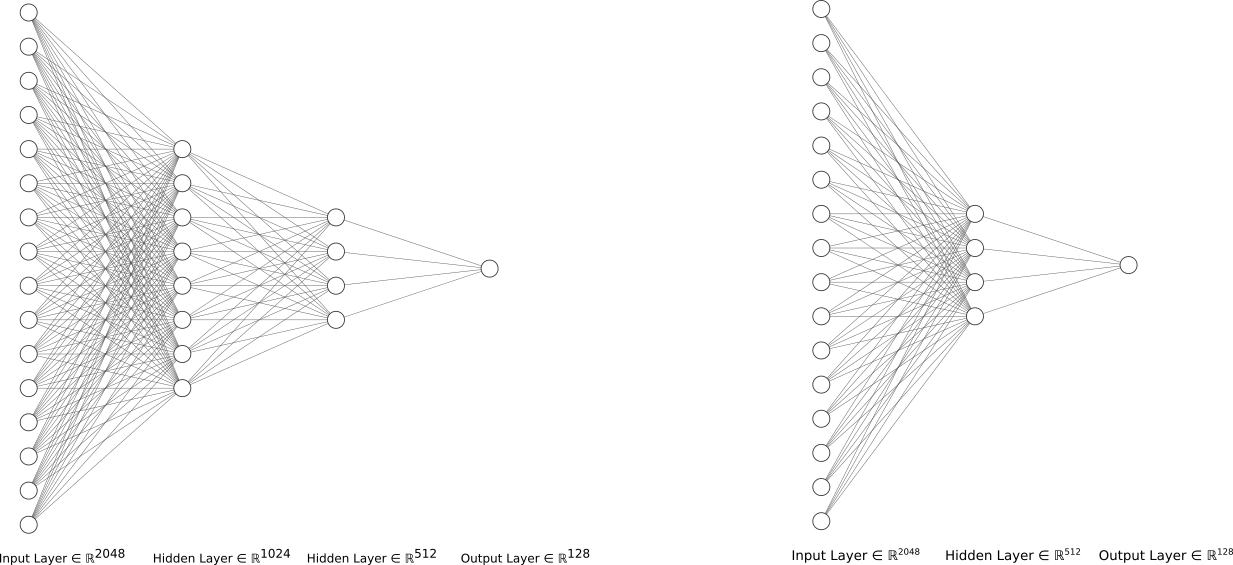
\includegraphics[width=0.8\textwidth]{Images/rl_architecture.png}
    \caption{TOBE CHANGED RL Framework Architecture: Actor-Critic Network}
    \label{fig:rlarchitecture}
\end{figure}

The \ac{RL} framework has been implemented using the \textit{Stable Baselines 3} library \cite{raffin_stable-baselines3_2021}. The \ac{RL} framework has been trained for $10$M steps, which given the episodic length, corresponds to $10$ epochs. The INSERT FIGURE below represents the main metrics collected in the training process. In particular the figure shows the mean reward, the mean episode length, the mean episodic reward, the approximated KL divergence and the explained variance.


\section{Evolutionary Algorithm Core}
\label{sec:EvolutionAlgo}

Evolutionary algorithm is a family of algorithms that are inspired by the natural selection
process, in which the fittest individuals are selected to reproduce and pass their genetic
material to the next generation.

The evolutionary algorithm has been used in the codesign loop to select motor parameters from a set of possible values. The evolutionary algorithm has been implemented using the \textit{DEAP} library CITE.

The motor set of parameters is composed of three main components: motor inertia, motor viscous friction and gear ratio. This choice has been made in order to keep the number of parameters low, in order to reduce the computational cost of the optimization process. The decision process is then repeated for each motor of the robot, which means that the total number of combination are:

\begin{equation}
    H = \binom{n + k - 1}{k} = \binom{23 + 3 - 1}{3} = \frac{25!}{3! 22!} = 2300
\end{equation}

where $n$ is the number of motors and $k$ is the number of parameters for each motor. In order to reduce the computational expense, we decided to focus on four crucial motors of the robot, which are the motors of the legs. This choice has been made because the legs are the main component of the robot that interacts with the environment, and therefore the choice of the motor parameters has a great impact on the performance of the robot. The total number of combinations is then reduced to:

\begin{equation}
    H = \binom{n + k - 1}{k} = \binom{4 + 3 - 1}{3} = \frac{6!}{3! 3!} = 20
\end{equation}

The evolutionary algorithm has been used to select the motor parameters from the set of possible values. The set of possible values for each parameter is shown in the \cref{tab:motorparams}.

\begin{table}[h]
    \centering
    \begin{tabular}{l c c c}
        \toprule
        \textbf{Motor} & \textsc{Inertia} $[k\mathrm{gm}^2]$ & \textsc{Gear Ratio} & \textsc{Viscous Friction} $[\mathrm{N}s\mathrm{rad}^{-1}]$ \\
        \midrule
        \textbf{S}     & $0.0001$                            & $1/100.0$           & $0.1$                                                      \\
        \textbf{M}     & $0.001$                             & $1/100.0$           & $0.15$                                                     \\
        \textbf{L}     & $0.001$                             & $1/160.0$           & $0.2$                                                      \\
        \bottomrule
    \end{tabular}
    \caption{Motor Set Parameters}
    \label{tab:motorparams}
\end{table}


After a preliminary analysis of the problem, the following parameters have been selected:

\begin{table}
    \centering
    \begin{tabular}{ll}
        \toprule
        \textbf{Parameter}    & \textbf{Value} \\
        \midrule
        Population Size       & $100$          \\
        Number of Generations & $100$          \\
        Crossover Probability & $0.5$          \\
        Mutation Probability  & $0.2$          \\
        \bottomrule
    \end{tabular}
    \caption{Evolutionary Algorithm Hyperparameters}
\end{table}

Given the single objective of the optimization problem, the \ac{NSGA}-III algorithm has been selected as the evolutionary algorithm, as it allows to find a set of solutions that are all Pareto optimal.


\section{Humanoid Robots Codesign Loop}
\label{sec:Codesign}

The problem of humanoid robot codesign can be formalized as a reinforcement learning problem, where the agent is the robot, together with a nonlinear optimization of some hardware parameters, in the case discussed in this work this role is played by a evolutionary algorithm.

The first step of the codesign loop involves some inital design choices, which are then used to create the initial population of the evolutionary algorithm. Then the population gets evaluated running in parallel the \ac{RL} framework for each individual of the population. The evaluation process is repeated for a number of generations, after which the best individual is selected and its parameters are used to update the robot design. The process is then repeated until the robot reaches the desired target fitness or when it reaches the maximum number of generations.

For the evaluation, the reward coming from the \ac{RL} training process is used as the fitness function of the evolutionary algorithm. The fitness function is then normalized to the range $[0,1]$ in order to make the optimization more stable.
